\documentclass[a4paper,11pt]{article}
\usepackage{minted}
\usepackage[utf8]{inputenc}
\usepackage{graphicx}
\usepackage{float}
\usepackage{subcaption}
\captionsetup[figure]{labelfont={bf, footnotesize} ,textfont={footnotesize, it}}
\captionsetup[subfigure]{labelfont={footnotesize, bf}, textfont=footnotesize,singlelinecheck=off,justification=raggedright}
\usepackage{amsmath}
\usepackage{amssymb}
\usepackage{geometry}
\usepackage{gensymb}
\usemintedstyle{borland}
\usepackage{ dsfont }
\usepackage{url}
\usepackage{hyperref}
\usepackage{listings}
\usepackage{color}
\setlength{\belowcaptionskip}{0pt}
\definecolor{mygreen}{RGB}{30,120,0}
\definecolor{mylilas}{RGB}{170,55,241}
\graphicspath{{img/}}

\title{\textbf{FHLF01} - Project}
\author{Johanna Gustafson \& Erik Lundell}
\date{}

\begin{document}
\lstset{language=Matlab,%
    %basicstyle=\color{red},
    breaklines=true,%
    morekeywords={matlab2tikz},
    keywordstyle=\color{blue},%
    morekeywords=[2]{1}, keywordstyle=[2]{\color{black}},
    identifierstyle=\color{black},%
    stringstyle=\color{mylilas},
    commentstyle=\color{mygreen},%
    showstringspaces=false,%without this there will be a symbol in the places where there is a space
    numbers=left,%
    numberstyle={\tiny \color{black}},% size of the numbers
    numbersep=9pt, % this defines how far the numbers are from the text
    emph=[1]{for,end,break},emphstyle=[1]\color{blue}, %some words to emphasise
    %emph=[2]{word1,word2}, emphstyle=[2]{style},    
}

\maketitle
a
\section{Introduction}
%Description of the problem, geometry and boundary conditions.
In this report a lens system on a Mars rover subjected to extreme temperature conditions is investigated. The shifting temperatures can cause significant deformation in the lenses and thus distort pictures taken through the lens. Analyzing this system to take sufficient precautions is therefore crucial for capturing high quality images from the rover.\\
\\The system is approximated as a flat disk with the thickness 1 cm, as shown in figure \ref{fig:geometry}. The two outermost lenses are curved as an ellipse with semi-axes 0.1 cm and 0.25 cm.

\begin{figure}[H]
    \centering
    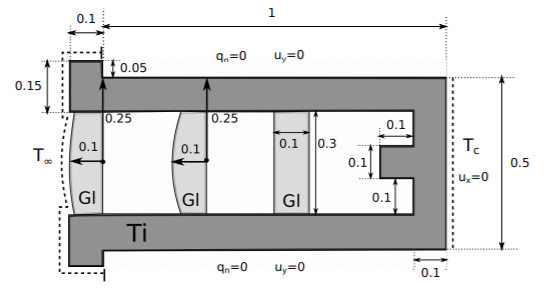
\includegraphics{geometri.png}
    \caption{The defined geometry of the lens system. All measurements in [cm] (image from project description).}
    \label{fig:geometry}
\end{figure}
\medskip \noindent Different properties hold for the materials of the structure as shown in table \ref{tab:material}.
\begin{table}[H]
    \centering
    \begin{tabular}{l l|c c}
         & & Titanium alloy & Glass \\ \hline
         Young's modulus, &  $E$ [GPa] & 110 & 67\\
         Poisson's ratio, & $\nu$ [-] & 0.34 & 0.2 \\
         Expansion coefficient, & $\alpha$ [1/K] & $9.4 \cdot 10^{-6}$ & $7\cdot 10^{-6}$\\
         Density, & $\rho$ [kg/m$^3$] & 4620 & 3860 \\
         Specific heat, & $c_p$ [J/(kg K)] & 523 & 670 \\
         Thermal conductivity, & $k$ [W/(m K)] & 17 & 0.8\\ \hline
    \end{tabular}
    \caption{Material data.}
    \label{tab:material}
\end{table}
\noindent The heat boundary condition for the inner boundaries is $q_n = 0$ as the spaces contain vacuum. The same condition holds for the top and bottom outer boundaries, whereas along the remaining outer boundaries there holds Newton convection; $q_n=\alpha_c(T-T_{\infty})$ along the left side and $q_n=\alpha_c(T-T_c)$ along the right, where $\alpha_c=100 \: \text{W}/(\text{m}^2 \text{K})$. The structure is stress-free at $20\degree$C.\\
\\The lens is mounted such that the top and bottom boundaries are fixated in the y-direction, meaning $u_y=0$. The rightmost boundary is fixated in the x-direction, meaning $u_x=0$. Remaining constraint-free boundaries are traction free, meaning $\boldsymbol{t}=\boldsymbol{0}$. Plane strain conditions are assumed to hold.\\
\\Because of symmetry, only the top half of the system must be analyzed, as the solution of the bottom half is identical, but mirrored. The new boundary condition along the middle edge must be $q_n = 0$ and $u_y = 0$ to conserve symmetry.\\
\\The report concerns two base cases for the outer temperature $T_{\infty}$. Day, where $T_{\infty} = 40\degree$C and night, where $T_{\infty} = -96\degree$C. The shift between the two temperatures is assumed to occur instantaneously. 

\section{Procedure}
%How the problems are solved (weak formulation, application of boundary conditions, treatment of thermal strains and so on). Derivation of the FE formulation and other important theoretical aspects should be included here. Note that you are encouraged to make references to textbooks. Though, it is important to carefully present all calculations that are not available in the literature.

The mesh was defined using MATLAB's \textit{pdetool} according to the specifications in figure \ref{fig:geometry}. The output were the points $\boldsymbol p$, edges $\boldsymbol e$ and triangles $\boldsymbol t$, that together define the geometry and general material properties of the structure. These were saved in a file \textit{data.mat}, which is loaded before any of the following steps.\\
\\The material properties are defined in the code of appendix \ref{kod:constants}, according to table \ref{tab:material}. Titanium is labeled 1 while glass is labeled 0 in order to automatically generate the correct constant for a certain element, using the method \textit{containers.Map()}.\\
\\The $\boldsymbol p$, $\boldsymbol e$ and $\boldsymbol t$ matrices are used to define the elements and \textit{edof}-matrix in CALFEM notation as seen in appendix \ref{kod:geometry}. Furthermore, edges are sorted according to their boundary condition. Edges are also labeled with either 1 or 0 in order to differentiate boundary conditions, in a similar fashion to that of material type.

\subsection{The stationary temperature distribution problem}
The Finite Element Formulation of the (2D) stationary temperature distribution problem is derived in Ottosen \& Petersson (1992). The method is derived using the strong formulation of the heat equation, 
\begin{equation} \label{eq:heatstrong}
    \nabla \cdot \boldsymbol q = Q
\end{equation}
and applying a constitutive law relating heat flux to temperature variations, 
\begin{equation}
    \boldsymbol q = -t\boldsymbol D\nabla T
\end{equation}
where $\boldsymbol{D}$ is the constitutive matrix, $Q$ denotes applied heat and $t$ the disc thickness. The temperature is approximated as $T=\boldsymbol{Na}$, where $\boldsymbol{a}$ contains the nodal temperatures, meaning
\begin{equation} \label{eq:heatflux}
    \boldsymbol{q} =-t \boldsymbol{D} \nabla \boldsymbol{Na} = -t \boldsymbol{DBa}.
\end{equation}

\bigskip \noindent Equation \ref{eq:heatstrong} is transformed to its weak form on the region $S$ with the boundary $\mathcal{L}$. The divergence theorem is used and equation \ref{eq:heatflux} is applied where appropriate. Finally the Galerkin method is applied, where the weight function $\boldsymbol{v} = \boldsymbol{Nc}$ and $\boldsymbol c$ is arbitrary, to reach
\begin{equation}
    \bigg ( \int_{S}\boldsymbol B^Tt\boldsymbol {DB} \: dS \bigg ) \boldsymbol a = -\oint_{\mathcal L}\boldsymbol N^Tq_nd \: \mathcal L + \int_S \boldsymbol N^T Qt \: dS,
\end{equation}
where $q_n$ is the heat flux normal to the boundary of the region. The value of $q_n$ depends on the boundary condition.\\
\\The boundary conditions on $\mathcal L$ can consist of
\begin{itemize}
    \item Dirichlet conditions (essential boundary conditions), where the temperature $T$ is given.
    \item Neumann conditions (natural boundary conditions), where the heat flow $q_n$ \textit{from} the body is given.
    \item Convection, where $q_n$ is given by Newton's heat equation: $q_n = \alpha(T-T_{\infty})$.
\end{itemize}

\noindent As mentioned in the introduction, the left- and rightmost boundaries have convection while the top and bottom boundaries, as well as the inner boundaries, are insulated, where $q_n = 0$. The problem can be further simplified as the thickness $t$ is constant, and as all materials are isomorphic so that $\boldsymbol D = k\boldsymbol I$. Finally $Q = 0$, resulting in the final formulation
\begin{align}
    t\int_A \boldsymbol B^T k \boldsymbol B dA \boldsymbol a = -\int_{\mathcal L_L} \boldsymbol N^T\alpha(T&-T_\infty)d\mathcal{L} -\int_{\mathcal L_R} \boldsymbol N^T\alpha(T-T_0)d\mathcal{L} \nonumber \\
    \bigg ( t\int_A \boldsymbol B^T k \boldsymbol B dA + \alpha\int_{\mathcal L_L + \mathcal L_R} \boldsymbol N^T\boldsymbol N d\mathcal{L} \bigg ) \boldsymbol a &= \alpha T_\infty\int_{\mathcal L_L} \boldsymbol N^T d\mathcal{L} + \alpha T_0\int_{\mathcal L_R} \boldsymbol N^T d\mathcal{L}\label{eq:final_stationary_temp}\\
    \iff \boldsymbol{(K+K_c)a} &= \boldsymbol f_{b_L} + \boldsymbol f_{b_R}\label{eq:long_notations}
\end{align}

\noindent where $\mathcal{L}_R$ refers to the outer right boundary and $\mathcal{L}_L$ the left. The notations $\boldsymbol{\Tilde{K}}$ and $\boldsymbol{\Tilde{f}}$ are introduced as
\begin{align}
    \boldsymbol{K+K_c} &= \boldsymbol{\Tilde{K}}\\
    \boldsymbol{f_{b_L}+f_{b_R}} &= \boldsymbol{\Tilde{f}}
\end{align}
to form the relation
\begin{equation}\label{eq:tildeKaf}
    \boldsymbol{\Tilde{K}a} = \boldsymbol{\Tilde{f}}.
\end{equation}

\medskip \noindent The boundary integrals of $\boldsymbol{K_c}$, $\boldsymbol{f_{b_L}}$ and $\boldsymbol{f_{b_R}}$ depend on the lengths of the edges along the boundaries. A single edge is located between the nearby nodes $i$ and $k$, wherein the form functions $N_i$ and $N_k$ are non-zero, and the rest 0. As a result, it is reasonable to analyze two form functions at a time.\\
\\Between the nodes $i$ and $k$, $N_i$ and $N_k$ take the form of linear functions, $u_i$ and $u_k$ respectively, for which $u_i: 1 \rightarrow 0$ and $u_k: 0 \rightarrow 1$. Letting $\mathcal{L'}$ denote the line between these nodes, and $l$ its length, it is found that
\begin{align}
    &\int_{\mathcal{L'}} \boldsymbol [N_i \quad N_k]^T \: d\mathcal{L'} = \int_0^l [u_i \quad u_{k}]^T \: d\mathcal{L'} = [l/2 \quad l/2]^T, \text{ and}
    \label{eq:bdry1}\\
    &\int_{\mathcal{L'}} \boldsymbol [N_i \quad N_k]^T \boldsymbol [N_i \quad N_k] \: d \mathcal{L'} = \int_0^l \begin{bmatrix}
    u_i^2 & u_i \cdot u_k\\
    u_i \cdot u_k & u_k^2
    \end{bmatrix} \: d\mathcal{L'} = \begin{bmatrix}l/3&l/6\\l/6&l/3\end{bmatrix}
    \label{eq:bdry2}
\end{align}
which are inserted into $\boldsymbol{K}_c$, $\boldsymbol{f}_{b_L}$ and $\boldsymbol{f}_{b_R}$ according to the nodal indices $i$ and $k$.

\subsubsection{MATLAB}
The code solution of this problem is shown in appendix \ref{kod:stationary}. The stiffness matrix $\boldsymbol K$ of equation \ref{eq:final_stationary_temp} is calculated elementwise using CALFEM's $flw2e.m$ to calculate the element stiffness matrices which are then assembled. $\boldsymbol{K}_c$ and $\boldsymbol{\Tilde{f}}$ are calculated using equations \ref{eq:bdry1} and \ref{eq:bdry2} to then form equation \ref{eq:tildeKaf}. The linear equation system is then complete and it is possible to solve for the nodal temperatures $\boldsymbol a$ using CALFEM's \textit{solveq.m}.

\subsection{The transient temperature problem}
The transient heat equation is similar to the stationary heat equation but contains an additional time derivative term,
\begin{equation}
    \rho c_p \dot T + \nabla 
    \cdot \boldsymbol q = Q.
    \label{eq:transHeatStrong}
\end{equation}
Introducing $\dot T = \boldsymbol{N} \dot{\boldsymbol{a}}$, the FE formulation the derivative term in equation \ref{eq:transHeatStrong} becomes
\begin{equation}
     \int_S \boldsymbol N^T  \rho c_p \boldsymbol N \: dS \cdot \dot {\boldsymbol a} = \boldsymbol A \dot{\boldsymbol a}
\end{equation}
resulting in the final equation
\begin{equation}
    \boldsymbol{\Tilde{K}a} + \boldsymbol{A\dot{a}} = \boldsymbol{\Tilde{f}},
    \label{eq:final_transient_heat}
\end{equation}
which is solved using a time-stepping method. In this project the implicit Euler method is used to allow for longer time steps without risking divergence. With the notation $\boldsymbol{a}^n = \boldsymbol{a}(t_n)$, the chosen method is defined as
\begin{equation}
    \boldsymbol{\dot a} =: \frac{\boldsymbol{ a^{n+1}} - \boldsymbol{ a^{n}}}{\Delta t} = g(\boldsymbol a^n),
\end{equation}
where $\Delta t$ is the length of the time step and $g$ is a given function. Inserting this definition into equation \ref{eq:final_transient_heat} and solving for $\boldsymbol{a^{n+1}}$ yields the closed form
\begin{equation}
    \boldsymbol{ a^{n+1}} = \big (\boldsymbol A + \Delta t \boldsymbol{\Tilde{K}} \big )^{-1} \big (\boldsymbol A \boldsymbol{ a^n} + \Delta t \boldsymbol{\Tilde{f}} \big ).
    \label{eq:time step}
\end{equation}

 \subsubsection{MATLAB}
 This time-stepping method requires an initial value $\boldsymbol{a}(0) = \boldsymbol{a}_0$, which is produced by running the solution for the stationary heat problem (appendix \ref{kod:stationary}), setting $T_{\infty}$ to either 20 $\degree$C or -96 $\degree$C depending on whether it initially is day- or nighttime. $\boldsymbol{\Tilde{f}}$ is recalculated using the temperature condition opposite to the initial condition.\\
 \\$\boldsymbol{A}$ is calculated elementwise using CALFEM's \textit{plantml.m}. The number of time-steps are chosen so that $\boldsymbol{a}$ is calculated for $t= $ 10, 100, 250 and 500 s.

\subsection{The mechanical problem}
Throughout the structure there are stresses present as a result of temperature variations and deformations. There are the normal stresses $\sigma_{xx}$, $\sigma_{yy}$ and $\sigma_{zz}$ in the $x$, $y$ and $z$ directions respectively, and the shear stresses $\tau_{jk}$ on the $j$ plane, in the $k$ direction. For the shear stresses it is found that $\tau_{xy}=\tau_{yx}$, $\tau_{xz}=\tau_{zx}$ and $\tau_{yz}=\tau_{zy}$ using moment equilibrium. Similar conditions hold for the normal strains $\varepsilon$ and shear strains $\gamma$.\\
\\For linear thermoelasticity, the relation between an element's stress and tension 
\begin{align*}
    \boldsymbol{\sigma} = \begin{bmatrix}
    \sigma_{xx}&
    \sigma_{yy}&
    \sigma_{zz}&
    \tau_{xy}&
    \tau_{xz}&
    \tau_{yz}
    \end{bmatrix}^T,&
    &\boldsymbol{\varepsilon} =
    \begin{bmatrix}
    \varepsilon_{xx}&
    \varepsilon_{yy}&
    \varepsilon_{zz}&
    \gamma_{xy}&
    \gamma_{xz}&
    \gamma_{yz}
    \end{bmatrix}^T
\end{align*}
is given by 
\begin{equation} \label{eq:sigeps}
    \boldsymbol{\sigma} = \boldsymbol{D (\varepsilon - \varepsilon_0)},
\end{equation}
where $\boldsymbol{D}$ is the constitutive matrix and $\boldsymbol{\varepsilon}_0$ is the initial strain. As there is plane strain, meaning $\varepsilon_{zz}=\gamma_{xz}=\gamma_{yz}=0$, it follows that $\sigma_{xz}=\sigma_{yz}=0$, and $\boldsymbol D$ and $\boldsymbol{\varepsilon}_0$ are consequently reduced in size. For an isotropic material, 
\begin{equation} \label{eq:D}
    \boldsymbol{D} = \frac{E}{(1+\nu)(1-2\nu)}\begin{bmatrix}
    1-\nu & \nu & 0 \\
    \nu & 1-\nu & 0\\
    0 & 0 & \frac{1}{2}(1-2\nu)\\
    \end{bmatrix}
\end{equation}
and the initial strain is given by
\begin{equation} \label{eq:epsilon02}
    \boldsymbol{\varepsilon_0} = (1+\nu)\alpha \Delta T \begin{bmatrix}
    1 & 1 & 0
    \end{bmatrix}^T.
\end{equation} 
The stress component $\sigma_{zz}$ has to be calculated separately through
\begin{equation} \label{eq:sigmazz}
    \sigma_{zz}=\frac{E \nu}{(1+\nu)(1-2\nu)}(\varepsilon_{xx}+ \varepsilon_{yy}) - \frac{\alpha E \Delta T}{1-2\nu}.
\end{equation}
\\
\\The differential equation of equillibrium is given by
\begin{equation}
    \boldsymbol{\Tilde{\nabla}\sigma + b} = \boldsymbol 0
\end{equation}
which gives rise to the weak formulation,
\begin{equation}
    \int_V (\boldsymbol{\Tilde{\nabla}v})^T \boldsymbol{\sigma} \: dV = \int_S \boldsymbol{v}^T\boldsymbol{t} \: dS + \int_V \boldsymbol{v}^T\boldsymbol{b} \: dV,
\end{equation}
where $\boldsymbol{b}$ is the force per unit volume and $\boldsymbol{t}$ is the traction vector.\\
\\The nodal displacement vector is given by $\boldsymbol{u} = \boldsymbol{Na}$, further meaning that $\boldsymbol{\varepsilon} = \boldsymbol{\Tilde{\nabla} u} = \boldsymbol{Ba}$. Using the Galerkin method, $\boldsymbol{v} = \boldsymbol{Nc}$, where $\boldsymbol{c}$ is arbitrary, and applying equation \ref{eq:sigeps} results in
\begin{equation} \label{eq:elasticFEM1}
    \bigg( \int_V \boldsymbol{B}^T\boldsymbol{DB} \: dV \bigg) \boldsymbol{a} = \int_S \boldsymbol{N}^T \boldsymbol{t} \: dS + \int_V \boldsymbol{N}^T \boldsymbol{b} \: dV + \int_V \boldsymbol{B}^T \boldsymbol{D \varepsilon_0} \: dV.
\end{equation}
As the structure is a flat disc with thickness $t$, equation \ref{eq:elasticFEM1} may be reduced to its 2D equivalent,
\begin{align}
    \bigg( \int_S \boldsymbol{B}^T\boldsymbol{DB} t \: dS \bigg) \boldsymbol{a} &= \oint_{\mathcal{L}} \boldsymbol{N}^T \boldsymbol{t} t \: d\mathcal{L} + \int_S \boldsymbol{N}^T \boldsymbol{b} t \: dS + \int_S \boldsymbol{B}^T \boldsymbol{D \varepsilon_0} t \: dS\\
    \iff \boldsymbol{Ka} &= \boldsymbol{f}_b + \boldsymbol{f}_l + \boldsymbol{f}_0. \label{eq:mechanicalFEM}
\end{align}
On the top and bottom boundaries $\mathcal{L}_T$ and $\mathcal{L}_B$ it is known that $u_y = 0$, and on the rightmost boundary $\mathcal{L}_R$ $u_x=0$. For the remaining components where the displacement is unknown, the traction is zero. Different properties hold for the different materials of the structure, meaning $S$ should be separated into $S_{Ti}$ for the titanium and $S_{Gl}$ for the glass. $\boldsymbol{b}=\boldsymbol{0}$ as there are no forces acting upon the structure. Thus,
\begin{align}
    \bigg( \int_S \boldsymbol{B}^T\boldsymbol{DB} t \: dS \bigg) \boldsymbol{a} &= \int_{\mathcal{L}_T + \mathcal{L}_B} \boldsymbol{N}^T \boldsymbol{t} t \: d\mathcal{L} + \int_{\mathcal{L}_R} \boldsymbol{N}^T \boldsymbol{t} t \: d\mathcal{L} \nonumber \\
    &+ \int_{S_{Ti}} \boldsymbol{B}^T (\boldsymbol{D \varepsilon_0})_{Ti} t \: dS + \int_{S_{Gl}} \boldsymbol{B}^T (\boldsymbol{D \varepsilon_0})_{Gl} t \: dS,
\end{align}
where appropriate values have been inserted into $\boldsymbol{a}$ and $\boldsymbol{t}$. As the known elements of $\boldsymbol{f}_b$ are 0, and the unknown elements aren't of interest, $\boldsymbol{f}_b$ may be ignored when solving the problem.\\
\\$\Delta T$ is in $\boldsymbol{f}_0$ (equation \ref{eq:mechanicalFEM}) integrated over the surface $S$, as $\boldsymbol{\varepsilon}_0$ is dependent of $\Delta T$ according to equation \ref{eq:epsilon02}. As $\Delta T$ varies linearly between nodes, we may conclude that
\begin{equation}\label{eq:meanT}
    \int_{S^e} \Delta T \: dS = S^e \cdot \frac{1}{3} \sum^3_{i=1} \Delta T_i
\end{equation}
meaning the integral over an element surface may be reduced to the product of the surface area and the mean of the nodal $\Delta T$.\\
\\\\The von Mises stress quantifies the total magnitude of the stress in a point and is defined as
\begin{equation}\label{eq:mises}
    \sigma_{eff} = \sqrt{\sigma_{xx}^2 + \sigma_{yy}^2 + \sigma_{zz}^2 + \sigma_{xx} \sigma_{yy} + \sigma_{xx} \sigma_{zz} + \sigma_{yy} \sigma_{zz} + 3 \tau_{xy}^2 + 3 \tau_{xz}^2 + 3 \tau_{yz}^2}
\end{equation}
which functions as a measure of effective stress on the structure. Because of the plane strain conditions, equation \ref{eq:mises} can be reduced to
\begin{equation}
    \sigma_{eff} = \sqrt{\sigma_{xx}^2 + \sigma_{yy}^2 + \sigma_{zz}^2 + \sigma_{xx} \sigma_{yy} + \sigma_{xx} \sigma_{zz} + \sigma_{yy} \sigma_{zz} + 3 \tau_{xy}^2}
\end{equation}
where $\sigma_{zz}$ is given by equation \ref{eq:sigmazz}.

\subsubsection{MATLAB}
The solution to the mechanical problem is presented in appendix \ref{kod:stress}. $\Delta T$ is known for each node by running the solution to the stationary temperature problem (appendix \ref{kod:stationary}) setting $T_{\infty}$ to either 20 $\degree$C or -96 $\degree$C depending on whether it is day- or nighttime. Then $\Delta T = T - 20 \: \degree$C.\\
\\The matrices $\boldsymbol K$ and $\boldsymbol{f}_0$ are generated using CALFEM's \textit{plante.m} and \textit{plantf.m} respectively, and equation \ref{eq:meanT} is used to calculate $\boldsymbol{D \varepsilon}_0$. The nodal component displacement vector $\boldsymbol{a}$ is then calculated using CALFEM's \textit{solveq.m}. The resulting $\boldsymbol{a}$ is then inserted as a parameter to CALFEM's \textit{plants.m} to retrieve $\boldsymbol{\sigma}$, excluding the contribution from the initial strain $\boldsymbol{\varepsilon}_0$, which is later added according to equations \ref{eq:sigeps}, \ref{eq:D} and \ref{eq:epsilon02}. As $\boldsymbol \sigma$ gives the stress of each element, the nodal von Mises stress is approximated as the mean of each connected element's von Mises stress.\\

\subsection{Displacement analysis}
To compare the magnitude of different distortions, the following quantity
\begin{equation}
    \int_S \boldsymbol u^T \boldsymbol u t \: dS = \boldsymbol a^T \int_S \boldsymbol N^T\boldsymbol N t \: dS \cdot \boldsymbol a,
    \label{eq:total_displacement}
\end{equation}
can be calculated, where $\boldsymbol{a}$ are the nodal component displacements in $\boldsymbol u = \boldsymbol{Na}$, calculated in the the mechanical problem above..

\subsubsection{MATLAB}
The solution is presented in appendix \ref{kod:displacement}. The nodal component displacements are retrieved by running the solution for the mechanical problem (appendix \ref{kod:stress}) with either day- or nighttime conditions. Equation \ref{eq:total_displacement} is calculated for displacements that are within the subdomain of the leftmost lens and then summed. Furthermore, the displacement of the whole structure is plotted.

\section{Results}
%Present the results in illustrative figures and/or tables. Note that the results should be commented such that the reader can not misunderstand the results (correct labels, units,figure texts etc.)

% EXERCISE A)
\subsection{Stationary temperature distribution}
The resulting stationary temperature distributions for the day and night case are shown in figure \ref{fig:stry_temp}. We see that the temperature in both cases changes gradually from one fixed temperature on one side to the other fixed temperature on the other side. There is no observable difference in behaviour between the titanium and glass materials. 

\begin{figure}[H]
    \centering
    \begin{subfigure}{0.45\linewidth}{
        \centering
        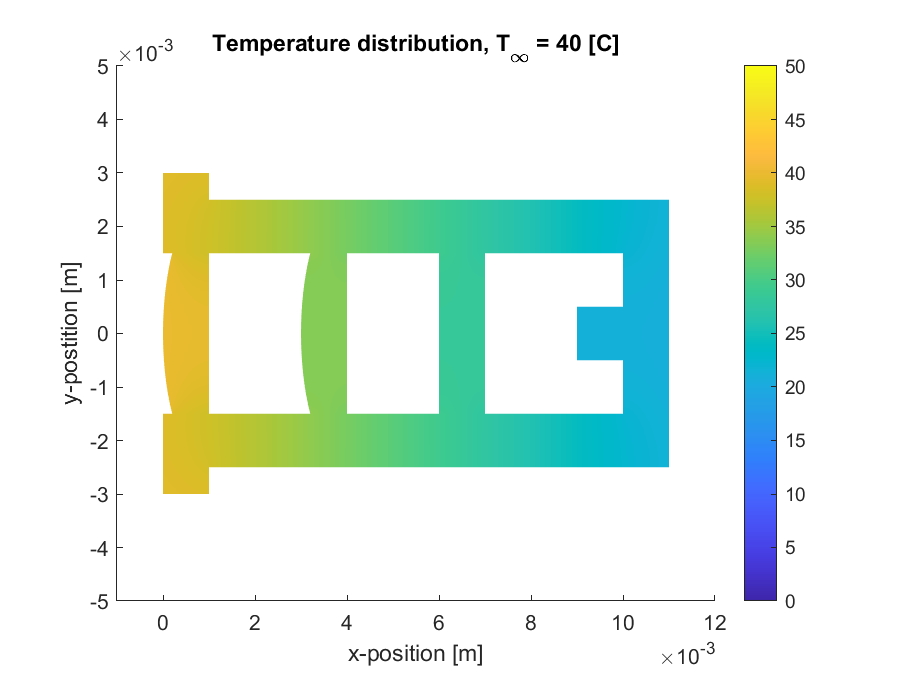
\includegraphics[width=1\linewidth]{aT40.eps}
        \caption{Stationary temperature distribution at daytime [$\degree$C]. Maximal calculated temperature: 39.954 $\degree$C}
        \label{fig:stry_temp_day}
    }\end{subfigure}
    \begin{subfigure}{0.45\linewidth}{
        \centering
        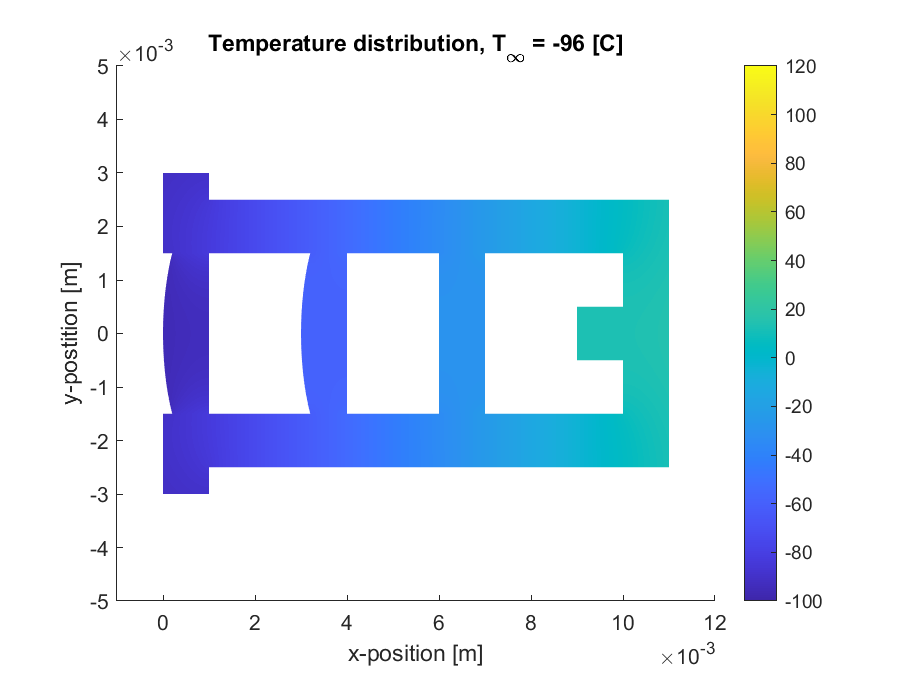
\includegraphics[width=1\linewidth]{aTminus96.eps}
        \caption{Stationary temperature distribution at nighttime [$\degree$C]. Maximal calculated temperature: 19,9769 $\degree$C}
        \label{fig:stry_temp_night}
    }\end{subfigure}
    \caption{Solutions to the stationary problem for different outside conditions. Note the different color scales.}
    \label{fig:stry_temp}
\end{figure}

% EXERCIES B)
\subsection{Transient temperature}
The results from when the boundary conditions switch from day to night conditions are shown in figure \ref{fig:trans_tempDN}. The results from when the boundary conditions switch from night to day conditions are shown in figure \ref{fig:trans_tempND}. As expected, in both cases the new temperature slowly seeps in from the left and spreads through the system. Over time the temperature distribution more and more resembles the stationary solution. We can observe different behaviour in the titanium and the glass material. In the titanium the heat spreads faster and diffuses, causing a soft gradient whereas the heat in the glass spreads slower and thus has a sharper gradient. The difference can be observed most clearly in figure \ref{sub:DN2} and \ref{sub:ND2}.

\begin{figure}[H]
    \centering
    \begin{subfigure}{0.45\linewidth}{
        \centering
        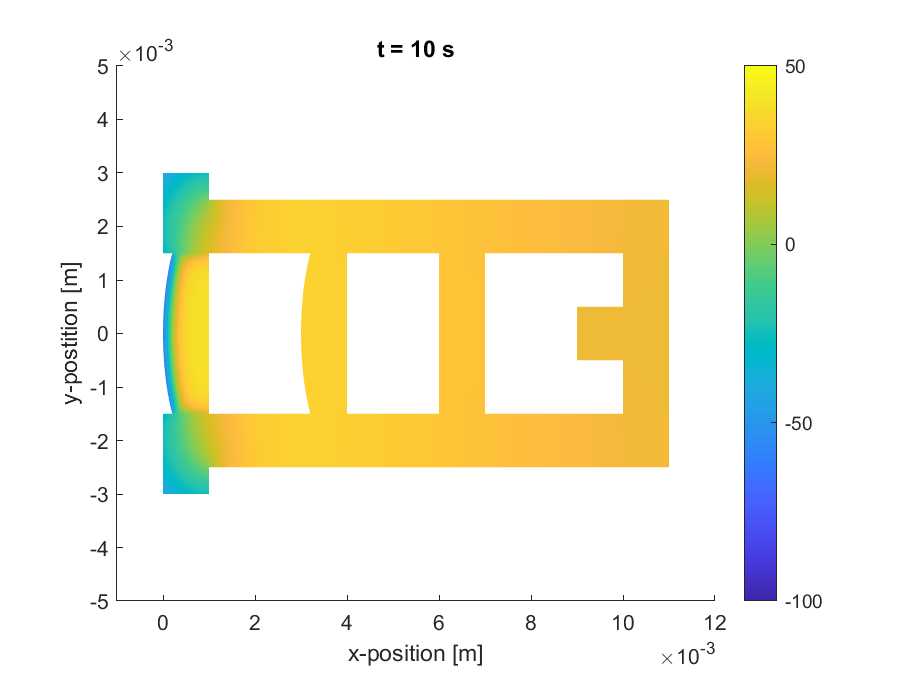
\includegraphics[width=1\linewidth]{bDN1.eps}
        \caption{Temperature distribution after 10\\seconds [$\degree$C].}
        \label{sub:DN1}
    }\end{subfigure}
    \begin{subfigure}{0.45\linewidth}{
        \centering
        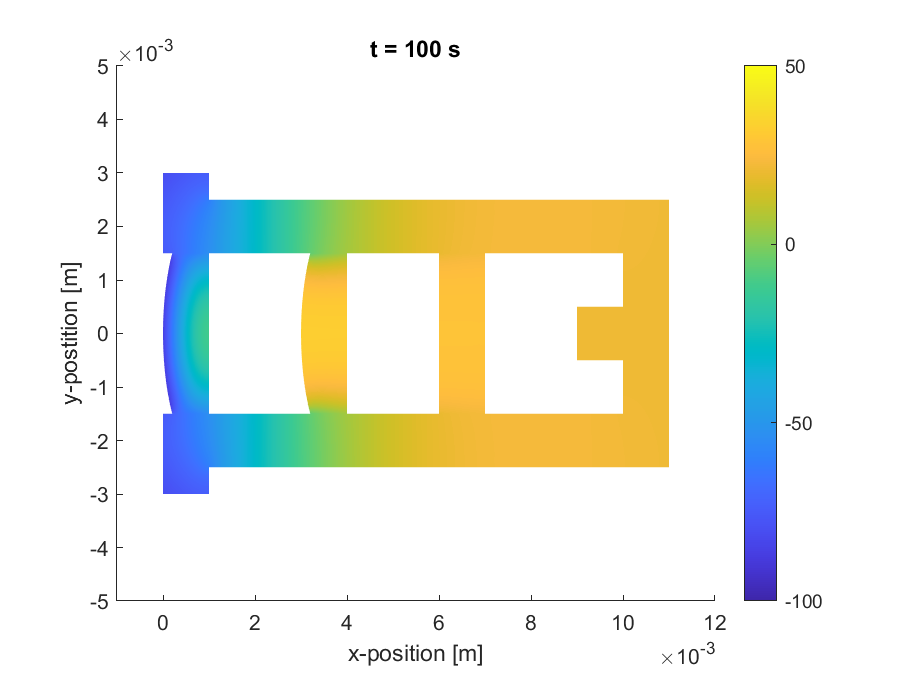
\includegraphics[width=1\linewidth]{bDN2.eps}
        \caption{Temperature distribution after 100 seconds [$\degree$C].}
        \label{sub:DN2}
    }\end{subfigure}
    \begin{subfigure}{0.45\linewidth}{
        \centering
        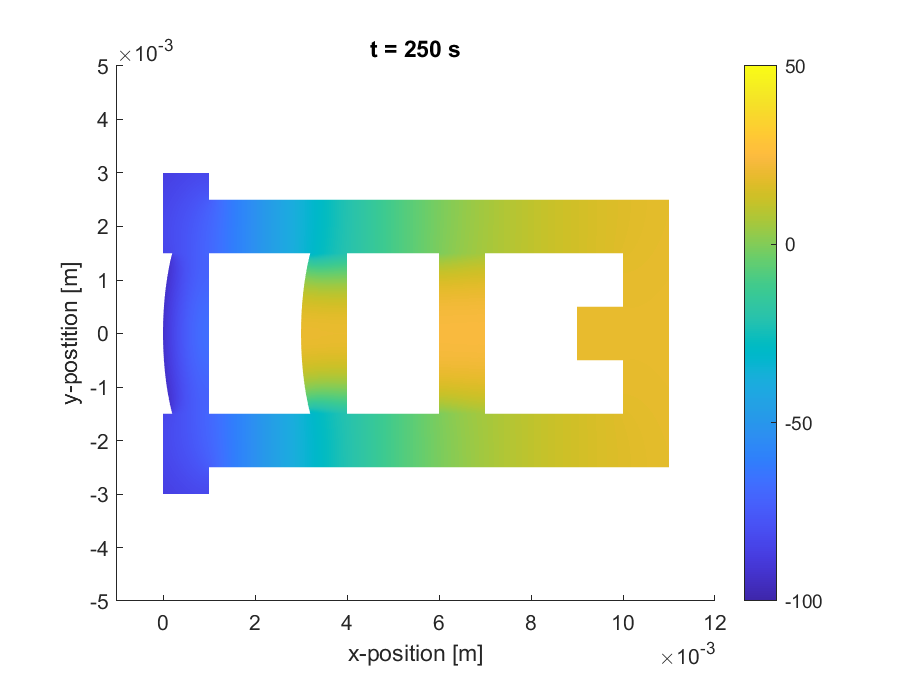
\includegraphics[width=1\linewidth]{bDN3.eps}
        \caption{Temperature distribution after 250 seconds [$\degree$C].}
        \label{sub:DN3}
    }\end{subfigure}
    \begin{subfigure}{0.45\linewidth}{
        \centering
        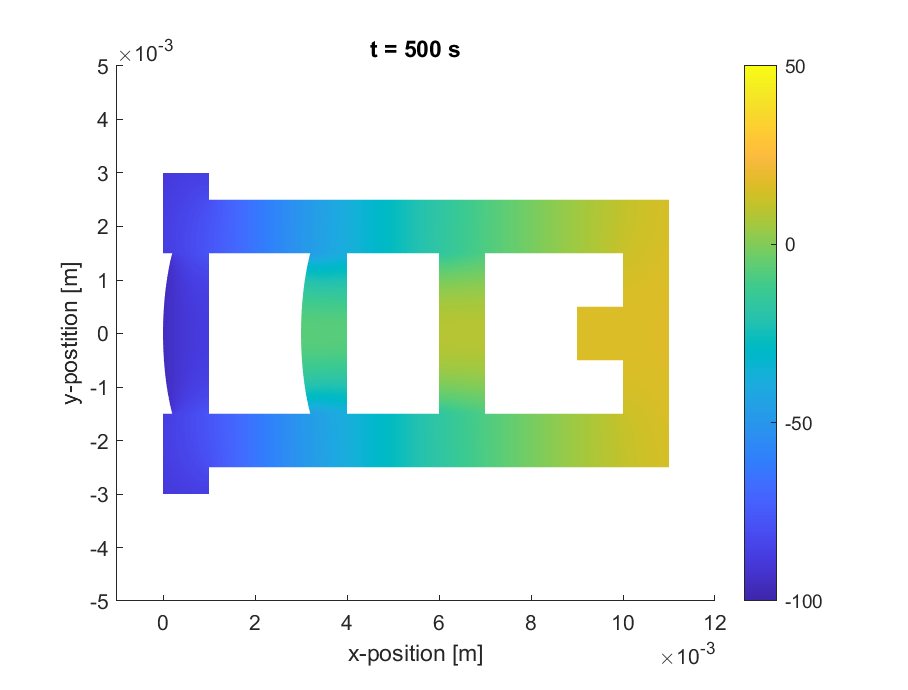
\includegraphics[width=1\linewidth]{bDN4.eps}
        \caption{Temperature distribution after 500 seconds [$\degree$C].}
        \label{sub:DN4}
    }\end{subfigure}
    \caption{Solutions to the transient heat problem, day to night.}
    \label{fig:trans_tempDN}
\end{figure}

\begin{figure}[H]
    \centering
    \begin{subfigure}{0.45\linewidth}{
        \centering
        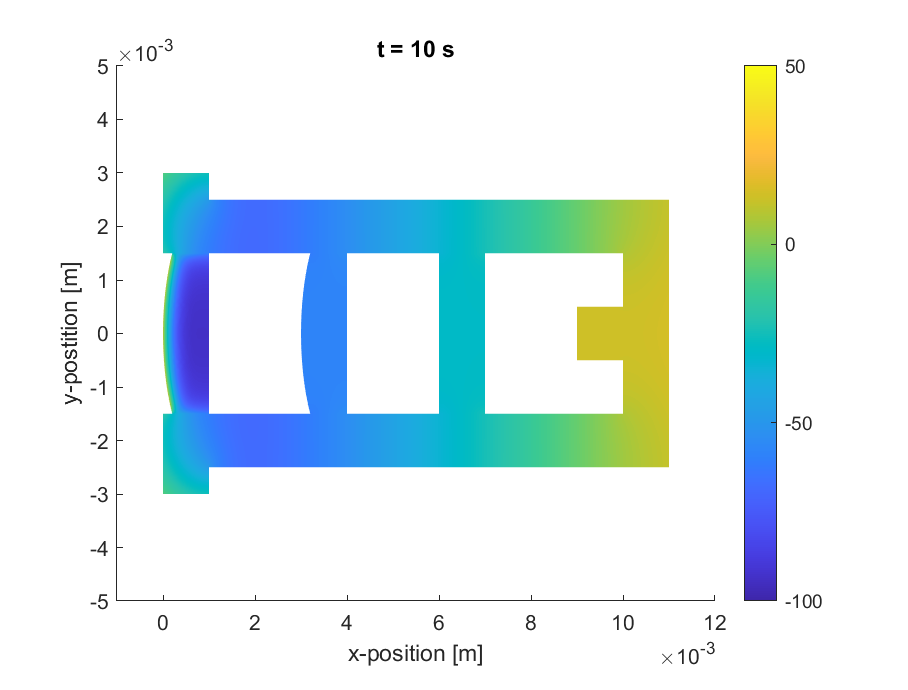
\includegraphics[width=1\linewidth]{bND1.eps}
        \caption{Temperature distribution after 10\\seconds [$\degree$C].}
        \label{sub:ND1}
    }\end{subfigure}
    \begin{subfigure}{0.45\linewidth}{
        \centering
        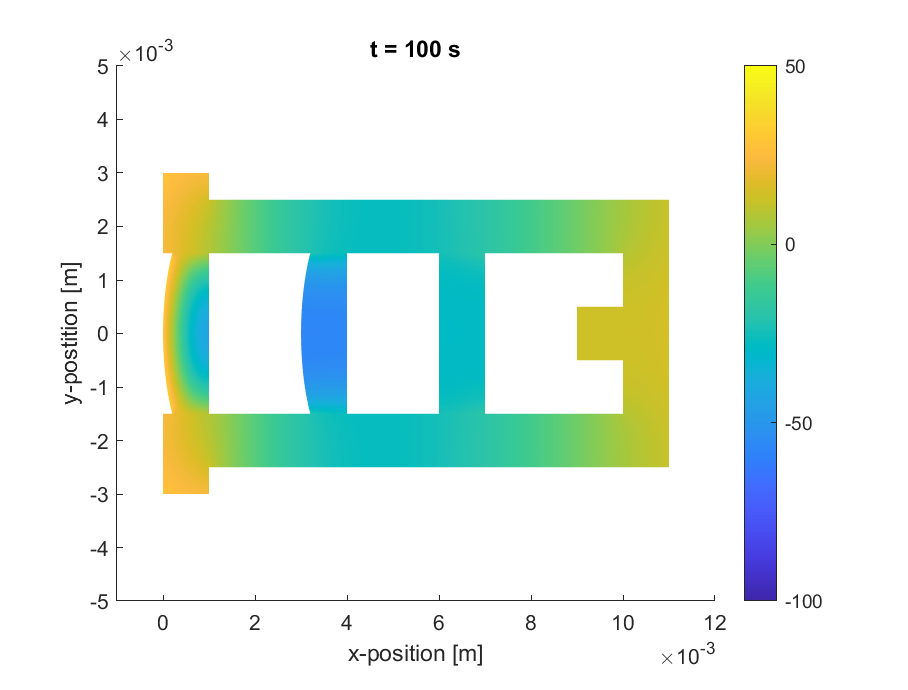
\includegraphics[width=1\linewidth]{bND2.eps}
        \caption{Temperature distribution after 100 seconds [$\degree$C].}
        \label{sub:ND2}
    }\end{subfigure}
    \begin{subfigure}{0.45\linewidth}{
        \centering
        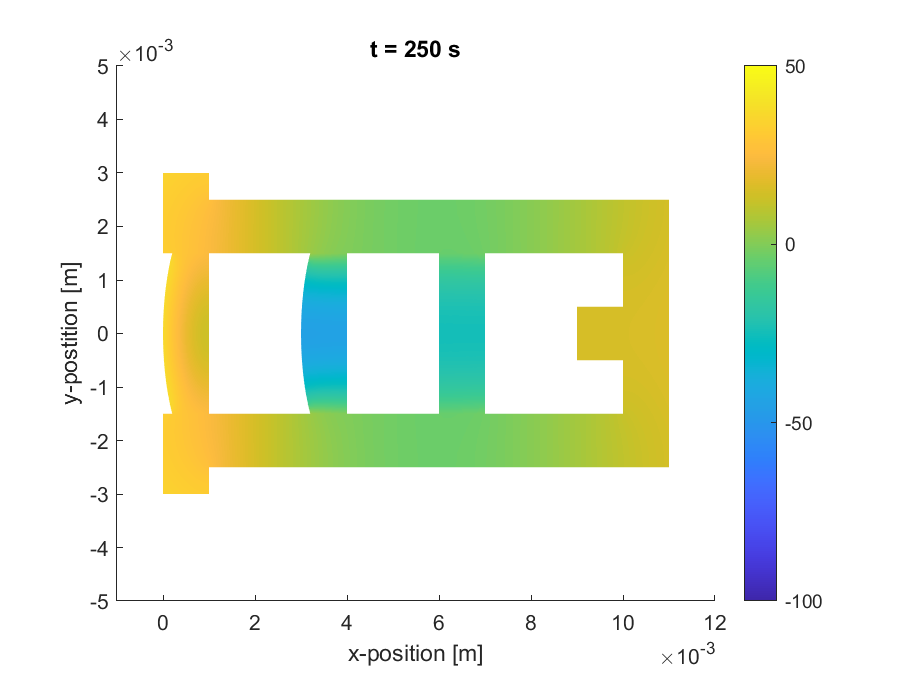
\includegraphics[width=1\linewidth]{BND3.eps}
        \caption{Temperature distribution after 250 seconds [$\degree$C].}
        \label{sub:ND3}
    }\end{subfigure}
    \begin{subfigure}{0.45\linewidth}{
        \centering
        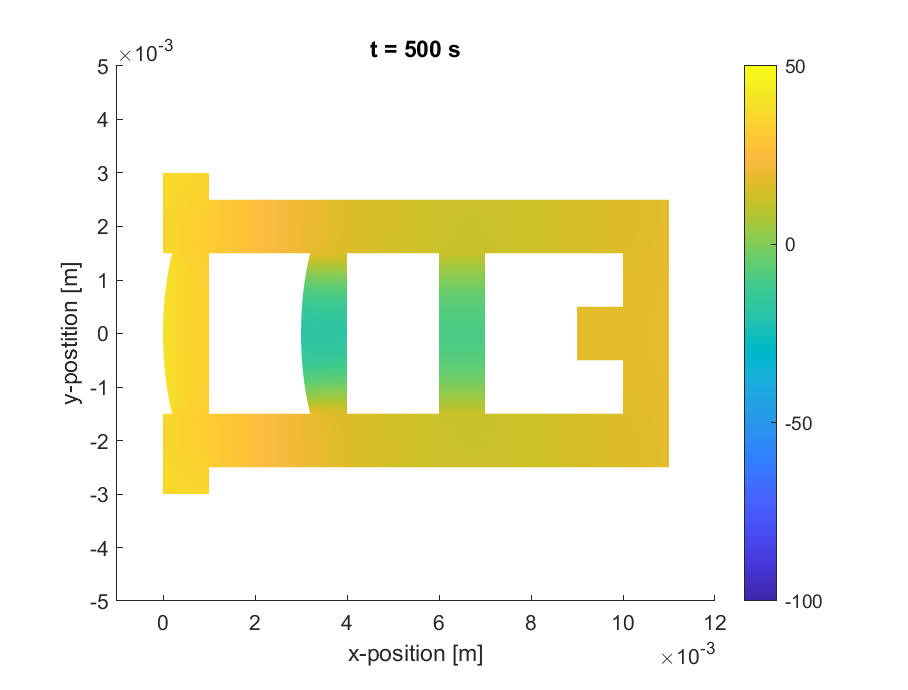
\includegraphics[width=1\linewidth]{bND4.eps}
        \caption{Temperature distribution after 500 seconds [$\degree$C].}
        \label{sub:ND4}
    }\end{subfigure}
    \caption{Solutions to the transient heat problem, night to day.}
    \label{fig:trans_tempND}
\end{figure}

\subsection{Body stresses}
The von Mises effective stress in the system for the two different conditions is shown in figure \ref{fig:cday} and \ref{fig:cnight}. The stresses appear to be equally distributed but of different magnitudes, the night conditions yielding stresses about 6-7 times larger than the day conditions. This is expected as the conditions too only differ in magnitude, where the night temperature is about 6 times further from $T_0$ than the day temperature. Whether the relation is linear is unknown. The main stresses are found on the edges of the left lens, where there is a sharp edge and where the lens is constrained by the metal body. The detailed view in figure for example \ref{sub:cday_detail} shows that the stresses vary quickly between elements which could indicate that the model and geometry is sensitive to the mesh shape.

\begin{figure}[H]
    \centering
    \begin{subfigure}{0.45\linewidth}{
        \centering
        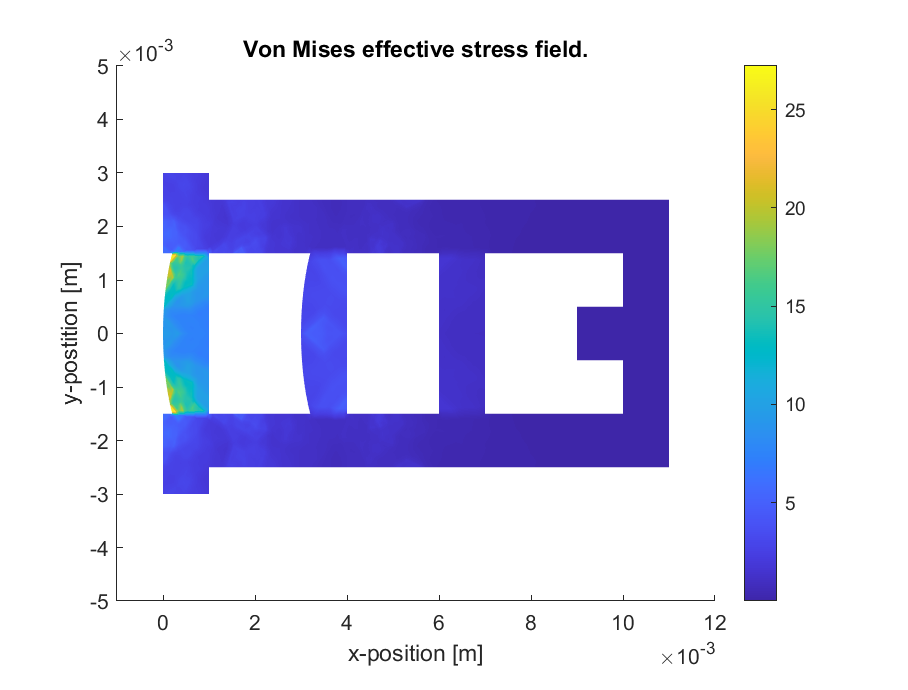
\includegraphics[width=1\linewidth]{cDay.eps}
        \caption{Complete view.}
        \label{sub:cday}
    }\end{subfigure}
    \begin{subfigure}{0.45\linewidth}{
        \centering
        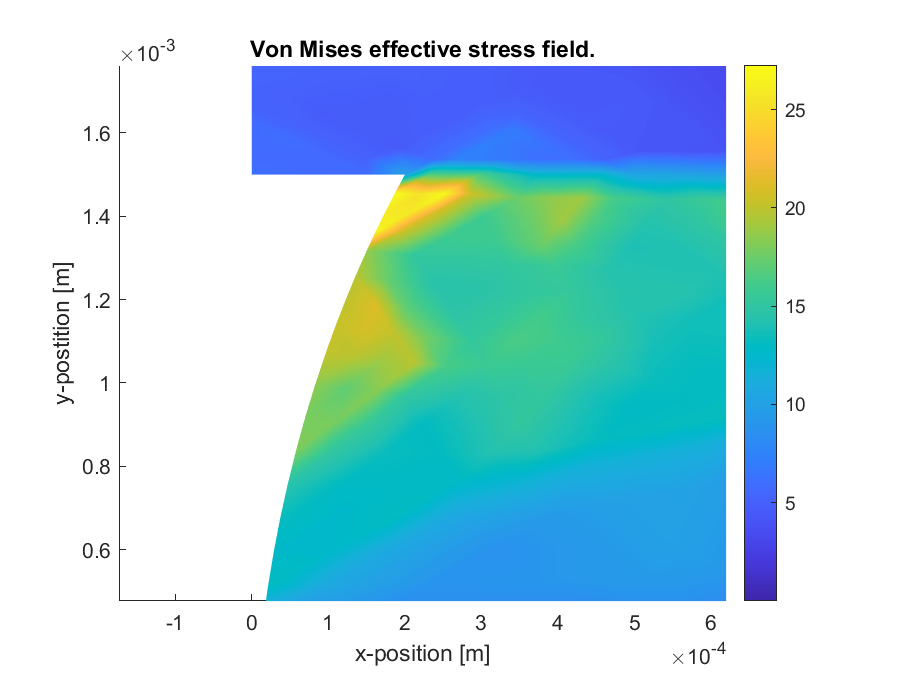
\includegraphics[width=1\linewidth]{cDayDetail.eps}
        \caption{Detailed view of top left lens-body border.}
        \label{sub:cday_detail}
    }\end{subfigure}
    \caption{The resulting von Mises effective stress field using the daytime condition [GPa].}
    \label{fig:cday}
\end{figure}

\begin{figure}[H]
    \centering
    \begin{subfigure}{0.45\linewidth}{
        \centering
        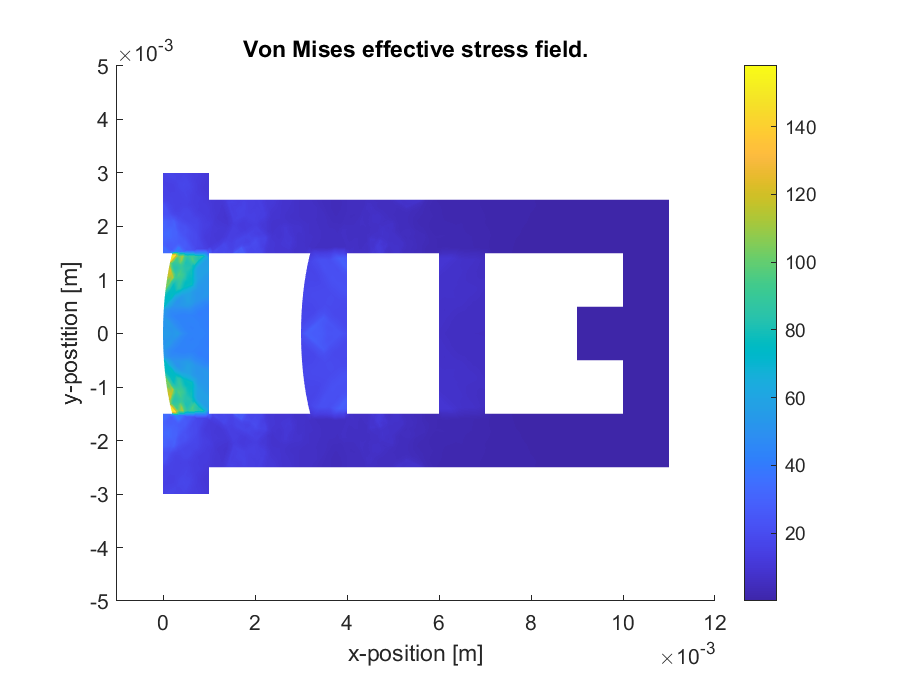
\includegraphics[width=1\linewidth]{cNight.eps}
        \caption{Complete view.}
        \label{sub:cnight}
    }\end{subfigure}
    \begin{subfigure}{0.45\linewidth}{
        \centering
        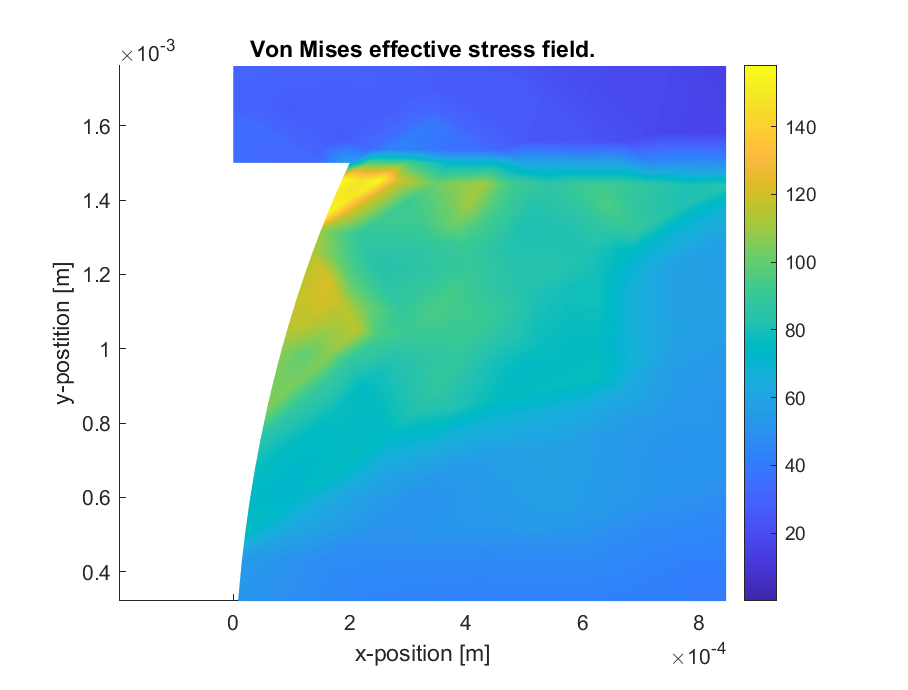
\includegraphics[width=1\linewidth]{cNightDetail.eps}
        \caption{Detailed view of top left lens-body border.}
        \label{sub:cnight_detail}
    }\end{subfigure}
    \caption{The resulting von Mises effective stress field using the nighttime condition [GPa].}
    \label{fig:cnight}
\end{figure}

\subsection{Node displacement}
The calculated displacements for the day and night conditions are plotted in figure \ref{eq:D}. As expected, the materials expand when heated and contract when cooled. The left side of the system is more distorted as it is closer to the boundary subjected to external heating. The titanium appears to distort more than the glass. We can also note that the night conditions cause a greater distortion which is due to being further from the stress free temperature. 
\\ \\
This can be confirmed by integrating the displacement function over all elements in the the left lens as described in equation \ref{eq:total_displacement}, yielding the following results:
\begin{itemize}
    \item Day conditions: 3.2339e-18
    \item Night conditions: 1.0879e-16
\end{itemize}
meaning that the night conditions cause distortions about 30 times larger.

\begin{figure}[H]
    \centering
    \begin{subfigure}{0.45\linewidth}{
        \centering
        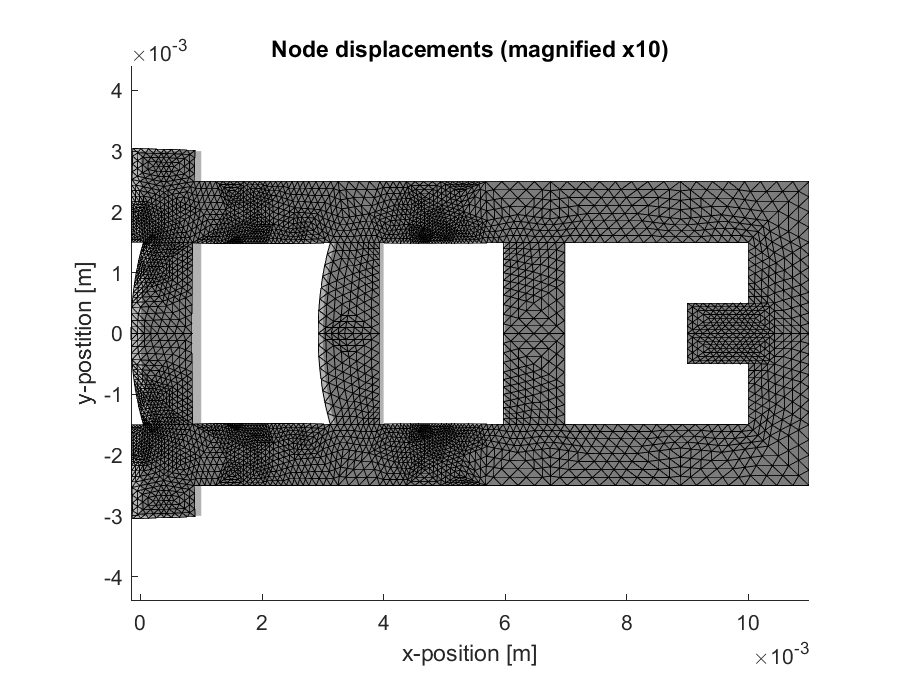
\includegraphics[width=1\linewidth]{dDay.eps}
        \caption{Resulting nodal displacements using the daytime condition.}
        \label{sub:dday}
    }\end{subfigure}
    \begin{subfigure}{0.45\linewidth}{
        \centering
        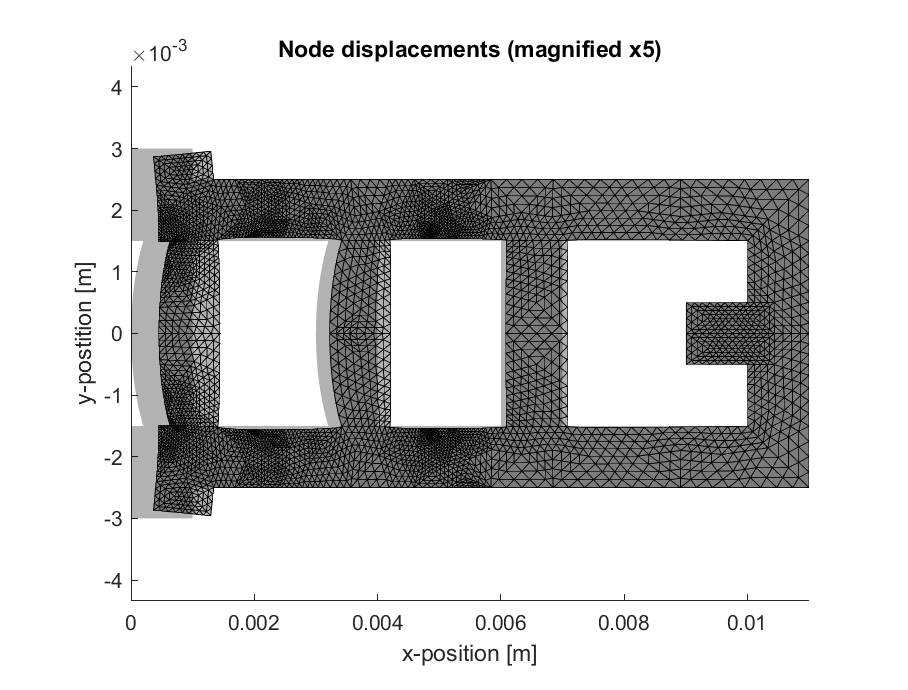
\includegraphics[width=1\linewidth]{dNight.eps}
        \caption{Resulting nodal displacements using the nighttime condition.}
        \label{sub:dnight}
    }\end{subfigure}
    \caption{Magnified nodal displacements. The grey silhouette presents the displacement-free structure. Note the different magnifications.}
    \label{fig:d}
\end{figure}

\section{Discussion}
%A discussion of the results, their meaning and significance. You might want to discuss sources of errors and accuracy in this section.

In this report a two-dimensional thermo-elastic system modelling a lens system in a mars rover has been analyzed using the Finite Element Method. The stationary temperature distributions for day and night conditions as well as the transient temperature distributions when changing between the two were calculated. The calculated temperature distributions were then used to analyze the stress and distortion in the system when subjected to the different conditions. The von Mises stress field and the nodal displacements were calculated, as well as a quantity describing the total displacement in the left lens.
\\ \\
The investigation has found that the left lens, especially the area around the boundary between the lens and the metal body, is subjected to both stress and and distortion. The stresses are equally distributed but of different magnitudes for different temperatures. However, the materials could both expand and contract depending on the temperature. The right boundary of the lens bends significantly in night conditions, as shown in figure \ref{sub:dnight}, which could cause distortions in the image taken through the lens. The titanium body appears to distort more whereas stresses build up in the glass lenses. This is explained by the different material parameters and is in line with our intuitive understanding of the two materials. Heat also diffuses faster in the metal compared to the glass.
\\ \\
A limitation of the model is the assumption that the materials remain elastic at all times. Especially close to the boundary between the left glass lens and the titanium body, the stresses were quite high and could potentially reach plasticity. Further investigations of the behaviour of the materials are needed to conclude whether this has to be accounted for in the model. 
\\ \\
To model the transient temperature more accurately, a continuous day-night has to be implemented. However, this would cause a slower temperature change which should allow the system to adapt slower. The abrupt switch between day and night used in this report could be used as a worst-case scenario when analyzing how the system reacts to changes in temperature.
\\ \\


\newpage

\appendix

\section{Computer code}
%Note that the code should be easy to follow and all declared variables should have intuitive names and be well commented.

\subsection{Material data} \label{kod:constants}
\lstinputlisting{kod/Constants.m}
\bigskip

\subsection{Geometry data}\label{kod:geometry}
\lstinputlisting{kod/MeshData.m}
\bigskip

\subsection{Stationary temperature}\label{kod:stationary}
\lstinputlisting{kod/StationaryTemp.m}
\bigskip

\subsection{Transient heat}\label{kod:transient}
\lstinputlisting{kod/TransientHeat.m} 
\bigskip

\subsection{Displacements and von Mises stress}\label{kod:stress}
\lstinputlisting{kod/MisesStress.m}
\bigskip

\subsection{Displacement field}\label{kod:displacement}
\lstinputlisting{kod/Displacement.m}
\bigskip

\subsubsection{Integral computation function}
\lstinputlisting{kod/NtN.m}


\end{document}
